% Template for ICASSP-2019 paper; to be used with:
%          spconf.sty  - ICASSP/ICIP LaTeX style file, and
%          IEEEbib.bst - IEEE bibliography style file.
% --------------------------------------------------------------------------
\documentclass{article}
\usepackage{spconf,amsmath,graphicx}
\usepackage{standalone}
\usepackage{tikz}
\usetikzlibrary{arrows.meta}
\usetikzlibrary{positioning}

% Example definitions.
% --------------------
\def\x{{\mathbf x}}
\def\L{{\cal L}}

% Title.
% ------
\title{Deep Learning for Acoustic Object Counting in Shaken Containers}
%
% Single address.
% ---------------
\name{Zhiheng Wang}
\address{School of Physics, Nanjing University}
%
% For example:
% ------------
%\address{School\\
%	Department\\
%	Address}
%
% Two addresses (uncomment and modify for two-address case).
% ----------------------------------------------------------
%\twoauthors
%  {A. Author-one, B. Author-two\sthanks{Thanks to XYZ agency for funding.}}
%	{School A-B\\
%	Department A-B\\
%	Address A-B}
%  {C. Author-three, D. Author-four\sthanks{The fourth author performed the work
%	while at ...}}
%	{School C-D\\
%	Department C-D\\
%	Address C-D}
%
\begin{document}
%\ninept
%
\maketitle
%
\begin{abstract}
In this paper, we attempt to articulate an approach to identify the number of small, identical items in an opaque container, solely relying on the sound it produces when shaken. This problem was proposed in IYPT 2024, and is of great practical value. It leverages the immense power of Deep Neural Network (DNN), specifically Convolutional Neural Network (CNN) in the time domain, a modern and popular method of digital signal processing for certain tasks. Our proposed model is ultra-lightweight, and can be trained and perform inference at ease with consumer-grade CPUs. Along with the model, we also present our experimental setup which we use to acquire the training and test data. Experimental results show our approach achieves superior performance and generalization ability. 
\end{abstract}
%
\begin{keywords}
Object Counting, Acoustic Signal Processing, Lightweight Model, Convolutional Neural Network
\end{keywords}

\section{INTRODUCTION}
\label{sec:intro}

This problem was among a list of 17 problems for the 37th IYPT 2024 and CUPT 2024 (China Undergraduate Physics Tournament), as they share the same set of problems; I attended the latter event two years ago. It was not the most popular problem by choice of the candidates, though, as it cannot be physically modeled in a traditional way. Looking back today, I thought it would be interesting to revisit the idea with the concept of deep learning and signal processing techniques. 

There have been significant breakthroughs in the fields of speech enhancement, music source separation and many other acoustic-signal-related fields, driven by the rapid development of deep learning techniques. Numerous model architectures were designed for multiple purposes, which take sound waveforms or spectrograms as their inputs; many of them were inspired by modern advances in CV. In our work, we similarly design a model with inspiration drawn from a classical CV model. 

Unlike the case with speech-related tasks, where high-quality datasets in large quantities are available online, such as the DNS challenge, VCTK Corpus and so on, our data is limited. The main reason is that our training data can only be obtained by our own experiments, as few researchers are solving the exact task we are tackling in this paper. The scarcity of data calls for proper regularization methods during the training of our model to avoid excessive overfitting in the training set. 

In this paper, we propose an 1-D CNN based model structure and an ordinal regression inspired loss function to identify the number of small, identical items in an opaque container, solely relying on the sound it produces when shaken. 

\section{DATA ACQUISITION}
\label{sec:data}

Training and test data are acquired with the apparatus shown in Fig.\ref{fig:exp}. The stepper motor is programmed and given instructions by an ESP-32 microcomputer on the Arduino platform. This guarantees that the container is rotated in a constant speed. Balls of two distinct materials, namely wood and silicon nitride, are used alternatively to validate the generalization ability of our approach. 

\begin{figure}[htb]

\begin{minipage}[b]{1.0\linewidth}
  \centering
  \centerline{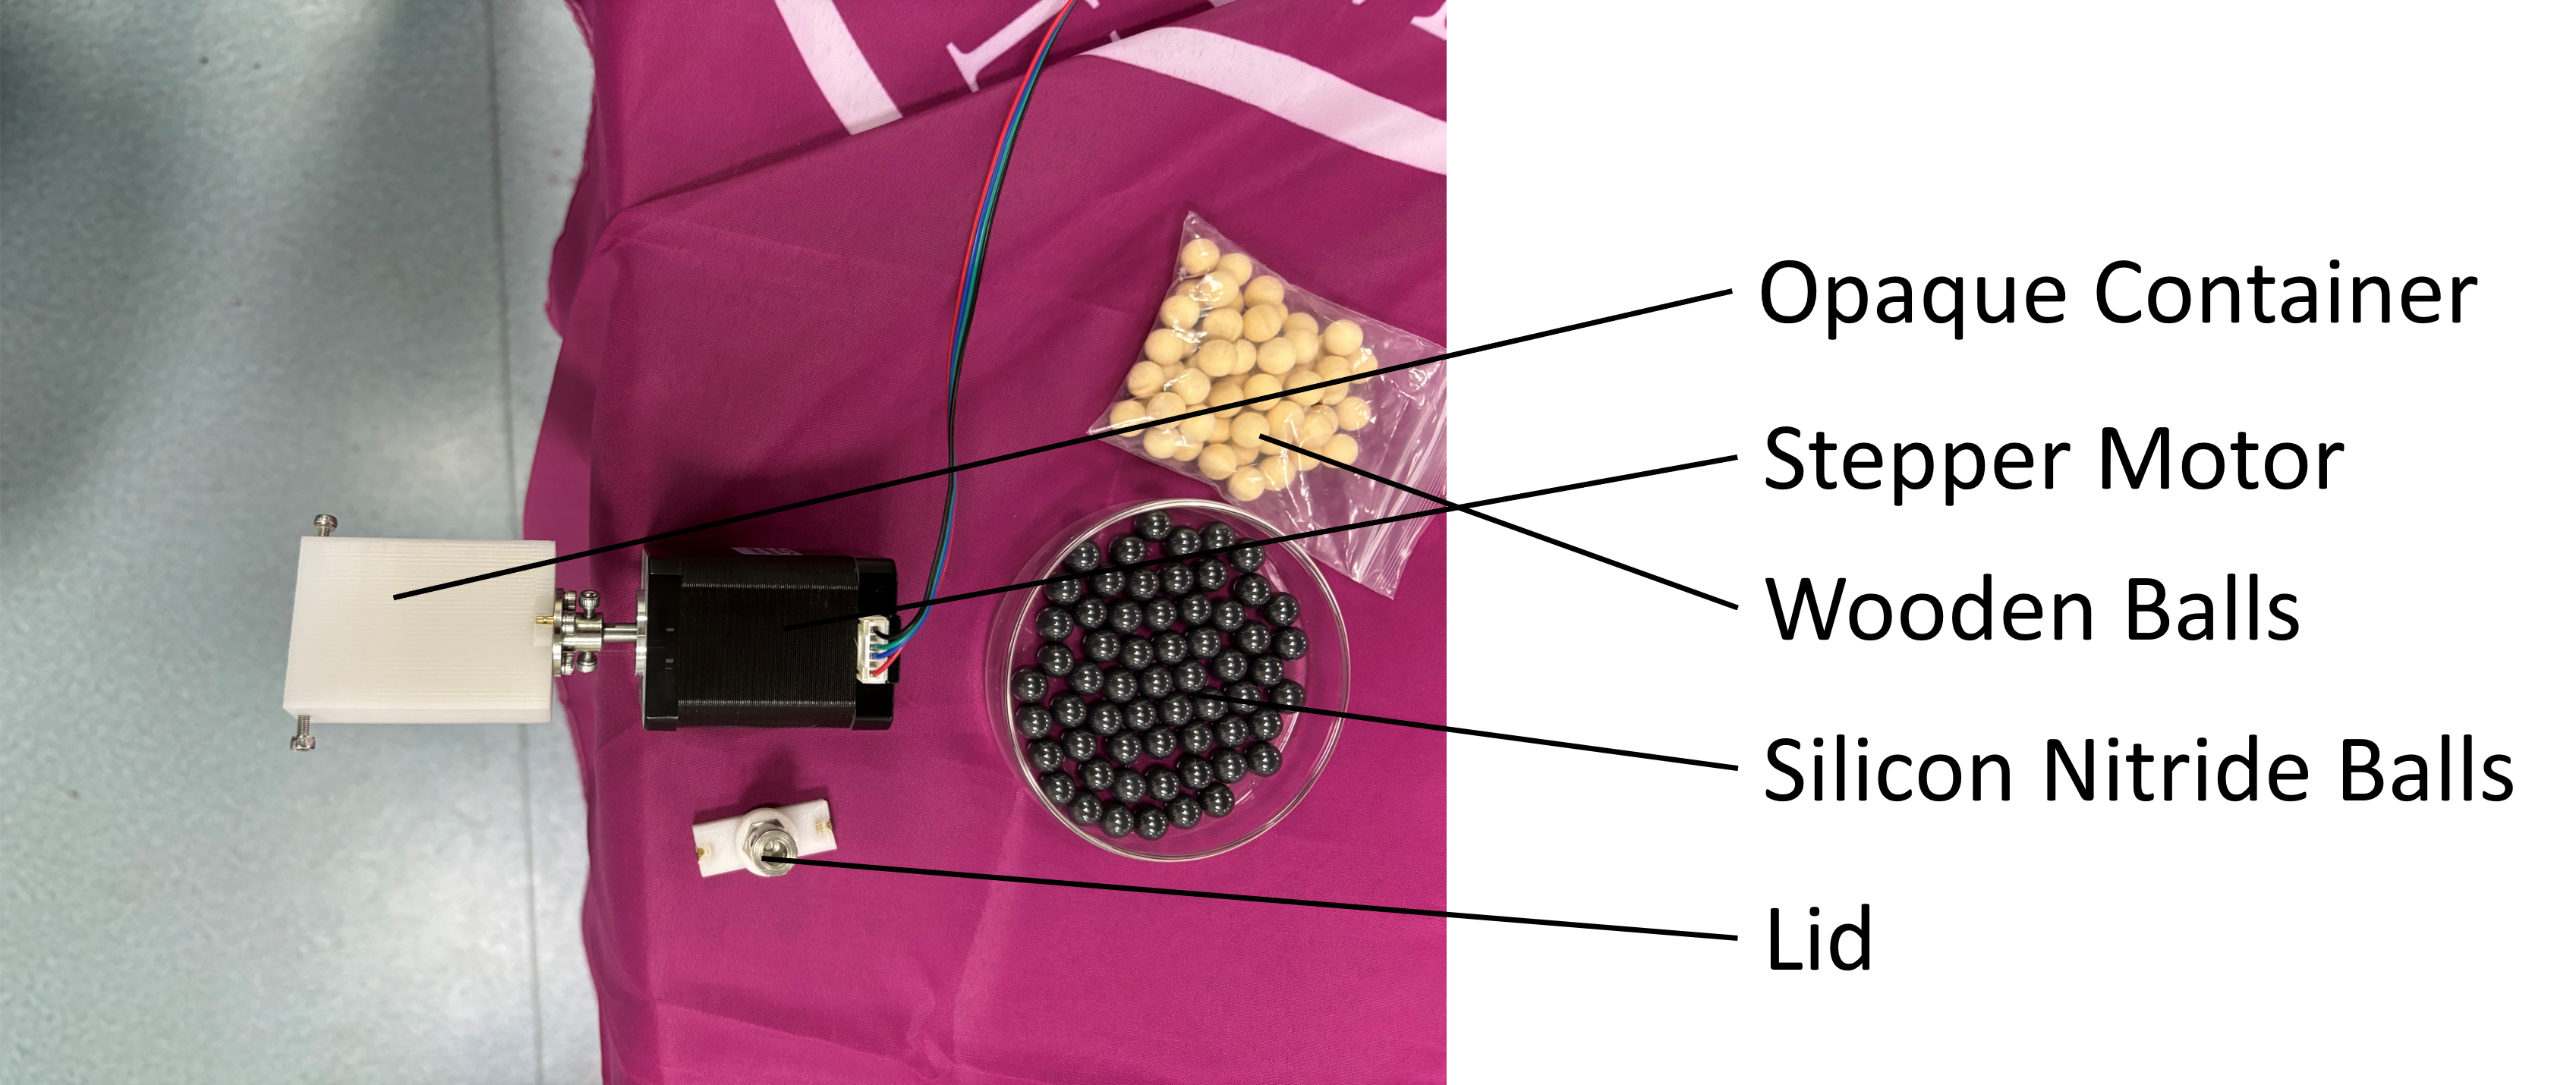
\includegraphics[width=8.5cm]{figs/exp.png}}
%  \vspace{2.0cm}
\end{minipage}
\caption{Experimental setup to acquire audio data. }
\label{fig:exp}
%
\end{figure}

Sound signals are collected at a distance by a directional microphone pointed to the container being shaken. The microphone has a rather flat frequency response curve (Fig.\ref{fig:freq}), operates at a sampling rate of 48 kHz, and picks up sound in a particular direction to filter out irrelevant noise.  

\begin{figure}[htb]

\begin{minipage}[b]{1.0\linewidth}
  \centering
  \centerline{\includegraphics[width=8.5cm]{figs/curve.png}}
%  \vspace{2.0cm}
\end{minipage}
\caption{Frequency response curve.}
\label{fig:freq}
%
\end{figure}

A total of 1.54 hours of data is collected with different types and numbers (1-15) of balls in the container, comprising of a balanced dataset. 

\section{MODEL ARCHITECTURE}
\label{sec:model}

\begin{figure}[htbp]

\begin{minipage}[b]{1.0\linewidth}
  \centering
  \centerline{\includegraphics[width=6cm]{figs/architecture.tex}}
%  \vspace{2.0cm}
\end{minipage}
\caption{Model architecture.}
\label{fig:model}
%
\end{figure}

Our model architecture consists of 1D convolutional blocks with ReLU activation, max-pooling modules and two fully-connected layers producing the output, which is supervised with ground-truth and an intricate loss function. An overview of our presented model is shown in Fig. \ref{fig:model}. Details of each module will be presented in the following sub-sections. 

\subsection{1D Convolution Blocks}

Scarce experimental data calls for a simple model configuration with fewer parameters. We draw our inspiration from the well-known LeNet-5, a lightweight document recognition model. It leverages the power of 2D convolution and subsampling to extract latent feature representation of the input data, an approach called representation learning. 

Here we replace 2D convolution with 1D convolution, since we are dealing with 1-dimensional input. We replace sigmoid activation with ReLU activation, subsampling layers with max-pooling layers as well, for these substitutions have proven more powerful theoretically and in DNN practices in the past few years. 

Convolutional layers with multiple channels can be seen as a set of filters, each capturing features in certain frequency bands. As data traverses deeper into the neural network, these filters are applied in a cascaded manner, and gradually extract abstract and high-level features while downsampling the time axis. Parameters within the filters are optimized in the training process. 

\subsection{Fully Connected Layers}

The output of the latent feature representation is, in turn, flattened and fed into fully connected layers. They facilitate information flow between channels and positions, and produce output logits. 

Dropout layers are inserted in this module with the aim of regularization, for fully connected layers consume a large number of parameters and may consequently result in overfitting. Dropout rate of $p=0.3$ is determined empirically. 

\subsection{Loss Function}

\section{MAJOR HEADINGS}
\label{sec:majhead}

Major headings, for example, "1. Introduction", should appear in all capital
letters, bold face if possible, centered in the column, with one blank line
before, and one blank line after. Use a period (".") after the heading number,
not a colon.

\subsection{Subheadings}
\label{ssec:subhead}

Subheadings should appear in lower case (initial word capitalized) in
boldface.  They should start at the left margin on a separate line.
 
\subsubsection{Sub-subheadings}
\label{sssec:subsubhead}

Sub-subheadings, as in this paragraph, are discouraged. However, if you
must use them, they should appear in lower case (initial word
capitalized) and start at the left margin on a separate line, with paragraph
text beginning on the following line.  They should be in italics.

\section{PRINTING YOUR PAPER}
\label{sec:print}

Print your properly formatted text on high-quality, 8.5 x 11-inch white printer
paper. A4 paper is also acceptable, but please leave the extra 0.5 inch (12 mm)
empty at the BOTTOM of the page and follow the top and left margins as
specified.  If the last page of your paper is only partially filled, arrange
the columns so that they are evenly balanced if possible, rather than having
one long column.

In LaTeX, to start a new column (but not a new page) and help balance the
last-page column lengths, you can use the command ``$\backslash$pagebreak'' as
demonstrated on this page (see the LaTeX source below).

\section{PAGE NUMBERING}
\label{sec:page}

Please do {\bf not} paginate your paper.  Page numbers, session numbers, and
conference identification will be inserted when the paper is included in the
proceedings.

\section{ILLUSTRATIONS, GRAPHS, AND PHOTOGRAPHS}
\label{sec:illust}

Illustrations must appear within the designated margins.  They may span the two
columns.  If possible, position illustrations at the top of columns, rather
than in the middle or at the bottom.  Caption and number every illustration.
All halftone illustrations must be clear black and white prints.  Colors may be
used, but they should be selected so as to be readable when printed on a
black-only printer.

Since there are many ways, often incompatible, of including images (e.g., with
experimental results) in a LaTeX document, below is an example of how to do
this \cite{Lamp86}.

\section{FOOTNOTES}
\label{sec:foot}

Use footnotes sparingly (or not at all!) and place them at the bottom of the
column on the page on which they are referenced. Use Times 9-point type,
single-spaced. To help your readers, avoid using footnotes altogether and
include necessary peripheral observations in the text (within parentheses, if
you prefer, as in this sentence).

% Below is an example of how to insert images. Delete the ``\vspace'' line,
% uncomment the preceding line ``\centerline...'' and replace ``imageX.ps''
% with a suitable PostScript file name.
% -------------------------------------------------------------------------
\begin{figure}[htb]

\begin{minipage}[b]{1.0\linewidth}
  \centering
  \centerline{\includegraphics[width=8.5cm]{image1}}
%  \vspace{2.0cm}
  \centerline{(a) Result 1}\medskip
\end{minipage}
%
\begin{minipage}[b]{.48\linewidth}
  \centering
  \centerline{\includegraphics[width=4.0cm]{image3}}
%  \vspace{1.5cm}
  \centerline{(b) Results 3}\medskip
\end{minipage}
\hfill
\begin{minipage}[b]{0.48\linewidth}
  \centering
  \centerline{\includegraphics[width=4.0cm]{image4}}
%  \vspace{1.5cm}
  \centerline{(c) Result 4}\medskip
\end{minipage}
%
\caption{Example of placing a figure with experimental results.}
\label{fig:res}
%
\end{figure}


% To start a new column (but not a new page) and help balance the last-page
% column length use \vfill\pagebreak.
% -------------------------------------------------------------------------
%\vfill
%\pagebreak

\section{COPYRIGHT FORMS}
\label{sec:copyright}

You must submit your fully completed, signed IEEE electronic copyright release
form when you submit your paper. We {\bf must} have this form before your paper
can be published in the proceedings.

\section{RELATION TO PRIOR WORK}
\label{sec:prior}

The text of the paper should contain discussions on how the paper's
contributions are related to prior work in the field. It is important
to put new work in  context, to give credit to foundational work, and
to provide details associated with the previous work that have appeared
in the literature. This discussion may be a separate, numbered section
or it may appear elsewhere in the body of the manuscript, but it must
be present.

You should differentiate what is new and how your work expands on
or takes a different path from the prior studies. An example might
read something to the effect: "The work presented here has focused
on the formulation of the ABC algorithm, which takes advantage of
non-uniform time-frequency domain analysis of data. The work by
Smith and Cohen \cite{Lamp86} considers only fixed time-domain analysis and
the work by Jones et al \cite{C2} takes a different approach based on
fixed frequency partitioning. While the present study is related
to recent approaches in time-frequency analysis [3-5], it capitalizes
on a new feature space, which was not considered in these earlier
studies."

\vfill\pagebreak

\section{REFERENCES}
\label{sec:refs}

List and number all bibliographical references at the end of the
paper. The references can be numbered in alphabetic order or in
order of appearance in the document. When referring to them in
the text, type the corresponding reference number in square
brackets as shown at the end of this sentence \cite{C2}. An
additional final page (the fifth page, in most cases) is
allowed, but must contain only references to the prior
literature.

% References should be produced using the bibtex program from suitable
% BiBTeX files (here: strings, refs, manuals). The IEEEbib.bst bibliography
% style file from IEEE produces unsorted bibliography list.
% -------------------------------------------------------------------------
\bibliographystyle{IEEEbib}
\bibliography{strings,refs}

\end{document}
